Az alkalmazás rendszer szinten mikroszerviz (\ref{sec:mikroszerviz}), a modulok szintjén hexagonális architektúrába (\ref{sec:hexagonalis_architektura}) rendezve készült el. A frontend Angulart (\ref{sec:angular}), a backend és az e-mail kliens Spring Boot-ot (\ref{sec:spring_boot}) használ.


\section{Mikroszerviz architektúra}\label{sec:mikroszerviz}
Bár a kifejezés már régóta ismert, nincs egy központilag elfogadott, egységes definíció arra nézve, miket nevezünk mikroszervizeknek. A legtöbb szerző jobb híján a visszatérő karakterisztikus tulajdonságuk alapján sorolja be az alkalmazásokat ebbe a kategóriába~\cite{OReally_Microservice_Architecture}. Egy tipikus mikroszerviz a következő tulajdonságoknak felel meg:

\begin{itemize}
	\item	pontosan egy üzleti funkció köré szerveződik 
	\item   más	szervizekkel laza, általában hálózaton keresztül megvalósuló kapcsolatban áll
	\item   ha szüksége van adatbázisra, akkor sajáttal rendelkezik
	\item	önmagában is működőképes	
	\item	decentralizált, tehát nincs egy a munkáját befolyásoló központi irányítórendszer
\end{itemize}

A hasonló felépítésükből adódóan, számos olyan eszköz van, ami --nem kötelezően, de legtöbbször-- együtt fordul elő a mikroszerviz architektúrával. A legfontosabb ilyen fogalmak a:
\begin{description}
	\item[skálázhatóság] a rendszer képessége az áteresztőképességének növelésére.
	Létezik vertikális\footnote{több processzor vagy memória bevonása} és horizontális skálázhatóság\footnote{újabb példányok futtatása}.
	
	\item[konténerizálás] a szerviz futtatása saját elszeparált környezetében hardveres virtualizáció segítsége nélkül.	

	\item[erőforrás felderítés] a rendszer által nyújtott erőforrások automatikus
	felfedezhetősége\footnote{angolul \textit{service discovery}-nek hívják}.
	
	\item[loadbalancer] az a folyamat, ami a bejövő feladatokat erőforrásokhoz rendeli. Legegyszerűbb megvalósítása a \foreignlanguage{british}{\textit{round robin}} algoritmus, célja a terhelés egyforma elosztása.
	
	\item[monitorozás] az önálló szervizek állapotának felügyelése. A monitorozás során nyújtott metrikák kiterjedhetnek a felhasznált memória mennyiségére, processzorigényére, vagy processzeire is.
\end{description}


\section{Hexagonális architektúra}\label{sec:hexagonalis_architektura}
A hexagonális architektúra --vagy más néven portok és adapterek architektúrája-- egy \foreignlanguage{british}{Alistair Cockburn} által létrehozott \cite{Alistair_Cockburn} szoftverterezési minta. Nevét a cikkben felrajzolt hatszögletű rendszerábrázolásról kapta (\ref{fig:Alistair_Cockburn_hexagonal_architecture} ábra), ami szembemegy a korábban elterjedt réteges elrendezéssel.

Az eredeti szándék mögötte az alkalmazás függetlenítése mindennemű külső függőségtől\footnote{például adatbázis, felhasználók, automatizált tesztek}, így lehetővé téve az üzleti és a technikai igények nagy mértékű szeparálását.
Egy absztrakt port feladata kell legyen a külvilággal való kapcsolat, így az üzleti logika csak az üzenet tartalmáért felelős, az üzenetküldés módjáért már nem.

\begin{figure}[hbt] 
	\centering
		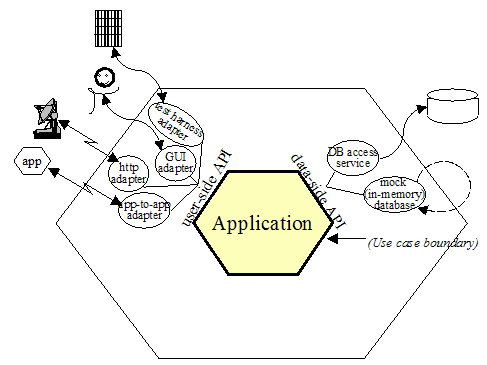
\includegraphics[width=0.85\textwidth]{Alistair_Cockburn_hexagonal_architecture.png}
	\caption[Hexagonális alkalmazások felépítése]{\foreignlanguage{british}{Alistair Cockburn} által \cite{Alistair_Cockburn} felrajzolt ábra a hexagonális alkalmazásról. Cockburn célja a külső függőségek elszeparálásának bemutatása.
}\label{fig:Alistair_Cockburn_hexagonal_architecture}
\end{figure}

Ahogy \foreignlanguage{british}{Robert C. Martin} a \foreignlanguage{british}{\textit{The Clean Architecture}} cikkében \cite{The_Clean_Architecture} összeszedte, a port-adapter és a hasonló architektúrával készülő alkalmazások mind:	
\begin{itemize}
	\item Könnyen, és önmagukban is tesztelhetőek. Mivel az üzleti szabályoknak, nincs külső függőségük.
	
	\item Függetlenek a külső tényezőktől. Így az alkalmazás által használt felület vagy adatbázis könnyen cserélhető.
	
	\item Keretrendszertől függetlenül is megvalósíthatóak. A megvalósítás nem függ semmilyen könyvtártól vagy egyéb tulajdonságtól.
\end{itemize}
	
	

\section{Event stream processing}
adatvezérelt, event based, szeparálás miatt 
publish subscribe
 schema
 kafka\\
event processiing általánosan?


\section{Rétegek szeparálása}\label{sec:retegek_szeparalasa}
A hexagonális architektúra (\ref{sec:hexagonalis_architektura} pont) és a hasonló \textit{clean code} \cite{clean_code_chapter_systems} elvek sokszor a különböző szoftver rétegek elkülönítésén alapszanak.


Hogy a feladatok elkülönítése ne vonzza magával az ismétlődő program részletek megnövekedését, célszerű a visszatérő, üzleti funkciót nem hordozó sorokat generálni. Ilyen --a fordítási időben-- kódot generáló eszközök a Mapstruct és a Lombok.


\section{Angular}\label{sec:angular}
Az \foreignlanguage{british}{Angular} egy a \foreignlanguage{british}{Google} által fejlesztett \foreignlanguage{british}{TypeScript} alapú platform és		 keretrendszer~\cite{angular_docs}. A segítségével létrehozott kód erősen modularizált, így könnyű vele újra felhasználható és az MVC-elveit követő alkalmazást létrehozni.

A segítségével készített honlap teljes mértében a kliens oldalon fut, így a szerver oldalon elegendő egy egyszerű, statikus HTML-oldalt visszaadó alkalmazásszerver használata.


\section{Spring Boot}\label{sec:spring_boot}
A \foreignlanguage{british}{Spring Boot} egy a Springre épülő keretrendszer. Mindkét rendszer alapja a függőség befecskendezése\footnote{Angolul \foreignlanguage{british}{\textit{Dependency Injection}}}, ami egy \aref{sec:retegek_szeparalasa} pontban említett tiszta kód \cite{clean_code_chapter_systems} eszköze.

A Spring Boot \cite{introducing_spring_boot} célja hogy gyorsan és egyszerűen lehessen önálló, magas minőségű alkalmazásokat fejleszteni:
\begin{itemize}
	\item az alapbeállítástól való eltérést kell meghatározni\footnote{A Spring Boot dokumentációban ezt röviden \textit{convention over configuration}-nek hívják} ezzel lecsökkentve a konfigurációval töltött időt,
	\item valamint sok gyakran visszatérő problémára\footnote{Például: metrikák, biztonság, adattárolás} nyújt könnyen elérhető megoldást.
\end{itemize}



